\chapter{Preliminaries and Related Work}
\label{ch:background}
\label{sec:related}
Inductive validity cores aim to bridge the gap between verification techniques and the user insight into the results provided by the tools. The goal behind this idea is to have expressive verification results that help the engineers to evaluate the quality of a system or specification.

This chapter, first, provides some formal background on symbolic model checking, which is the underlying method for IVC generation. Broadly, IVCs can be compared with several existing methods such as invariant minimization, minimal unsatisfiable subformula, and slicing. We compare IVCs with these techniques in this chapter. Several major uses of IVCs are in requirements traceability, checking adequacy and vacuity. This chapter also discusses existing approaches in the literature used for these purposes.



\section{Symbolic Model Checking}

The idea of inductive validity cores is applicable to the context of symbolic model checking using inductive proof methods. After proving the correctness of a given property, we extract a minimal portion of the system (model) necessary for the proof of the property, which is what we call IVCs.
Correctness can be expressed in terms of \emph{safety} and \emph{liveness} properties. Safety properties state that nothing bad ever happens, while liveness properties specifying that something good eventually happens.

IVCs determine why a \emph{safety} property is satisfied by the system. Since this information is obtained from the inductive proofs, we call it \emph{inductive} validity core. With minimal IVCs, we are able to abstract away the part of the system irrelevant to the proof of the property. This section mentions some background on symbolic model checking.

Given a state space $U$, a transition system $(I,T)$ consists of an
initial state predicate $ I : U \to \bool $ and a transition step
predicate $ T : U \times U \to \bool $.
We define the notion of
reachability for $(I, T)$ as the smallest predicate $\reach : U \to
\bool$ which satisfies the following formulas:

\begin{gather*}
  \forall u.~ I(u) \Rightarrow \reach(u) \\
  \forall u, u'.~ \reach(u) \land T(u, u') \Rightarrow \reach(u')
\end{gather*}

A safety property $P : U \to \bool$ is a state predicate. A safety
property $P$ holds on a transition system $(I, T)$ if it holds on all
reachable states, i.e., $\forall u.~ \reach(u) \Rightarrow P(u)$,
written as $\reach \Rightarrow P$ for short. When this is the case, we
write $(I, T)\vdash P$.

For an arbitrary transition system $(I, T)$, computing reachability
can be very expensive or even impossible. Thus, we need a more
effective way of checking if a safety property $P$ is satisfied by the
system. The key idea is to over-approximate reachability. If we can
find an over-approximation that implies the property, then the
property must hold. Otherwise, the approximation needs to be refined.

A good first approximation for reachability is the property itself.
That is, we can check if the following formulas hold:
\begin{gather}
  \forall u.~ I(u) \Rightarrow P(u)
  \label{eq:1-ind-base} \\
  \forall u, u'.~ P(u) \land T(u, u') \Rightarrow P(u')
  \label{eq:1-ind-step}
\end{gather}
If both formulas hold then $P$ is {\em inductive} and holds over the
system. If (\ref{eq:1-ind-base}) fails to hold, then $P$ is violated
by an initial state of the system. If (\ref{eq:1-ind-step}) fails to
hold, then $P$ is too much of an over-approximation and needs to be
refined.

One way to refine our over-approximation is to add additional lemmas
to the property of interest. For example, given another property $L :
U \to bool$ we can consider the extended property $P'(u) = P(u) \land
L(u)$, written as $P' = P \land L$ for short. If $P'$ holds on the
system, then $P$ must hold as well. The hope is that the addition of
$L$ makes formula (\ref{eq:1-ind-step}) provable because the
antecedent is more constrained. However, the consequent of
(\ref{eq:1-ind-step}) is also more constrained, so the lemma $L$ may
require additional lemmas of its own. Finding and proving these
lemmas is the means by which property directed reachability (PDR)
strengthens and proves a safety property~\cite{Een2011:PDR}.

Another way to refine our over-approximation is to use use {\em
  $k$-induction} which unrolls the property over $k$ steps of the
transition system. For example, 1-induction consists of formulas
(\ref{eq:1-ind-base}) and (\ref{eq:1-ind-step}) above, whereas
2-induction consists of the following formulas:
\begin{gather*}
\forall u.~ I(u) \Rightarrow P(u) \\
\forall u, u'.~ I(u) \land T(u, u') \Rightarrow P(u') \\
\forall u, u', u''.~ P(u) \land T(u, u') \land P(u') \land T(u',
  u'') \Rightarrow P(u'')
\end{gather*}
That is, there are two base step checks and one inductive step check.
In general, for an arbitrary $k$, $k$-induction consists of $k$
base step checks and one inductive step check as shown in
Figure~\ref{fig:k-induction} (the universal quantifiers on $u_i$ have
been elided for space). We say that a property is $k$-inductive if it
satisfies the $k$-induction constraints for the given value of $k$.
The hope is that the additional formulas in the antecedent of the
inductive step make it provable.
In practice, inductive model checkers often use a combination of the
above techniques. Thus, a typical conclusion is of the form ``$P$ with
lemmas $L_1, \ldots, L_n$ is $k$-inductive''.

\begin{figure}
\begin{gather*}
I(u_0) \Rightarrow P(u_0) \\[-2pt]
%
\vdots \\[2pt]
%
I(u_0) \land T(u_0, u_1) \land \cdots \land T(u_{k-2}, u_{k-1})
\Rightarrow P(u_{k-1}) \\[2pt]
%
P(u_0) \land T(u_0, u_1) \land \cdots \land P(u_{k-1}) \land
T(u_{k-1}, u_k) \Rightarrow P(u_k)
\end{gather*}
\caption{$k$-induction formulas: $k$ base cases and one inductive
  step}
\label{fig:k-induction}
\end{figure}


%%% Local Variables:
%%% mode: latex
%%% TeX-master: "main.tex"
%%% End

%%  LocalWords:  bool reachability \texttt{JKind} Lustre PDR Yices MathSAT ok
%%  LocalWords:  SMTInterpol dataflow init

Unbounded model checking is performed through inductive proof methods such as $k$-induction~\cite{SheeranSS00} and IC3/PDR~\cite{Een2011:PDR}.
The PDR is currently the dominant unbounded model checking technique. In the past few years, several variations of this algorithm have been published \cite{hoder2012generalized, vizel2014interpolating, jovanovic2016property, gurfinkelk}.
The original idea in PDR is to compute  a
safe  inductive  invariant by strengthening the property using inductive couter-examples without unrolling the transition relation, while a classical implementation of
$k$-induction tries to find an inductive invariant through
$k$-step unrolling of a transition relation. Symbolic model checkers usually employ these proof methods, using an SMT/SAT solver in the backend. For example, \texttt{JKind} \cite{jkind} is an SMT-based model checker for safety properties that uses parallel cooperating engines including $k$-induction, PDR, and template-based invariant generation.

Another form of symbolic evaluation is performed through bounded model checking.
The goal of bounded model checking is to decide if a given program reaches an error within at
most $k$ unfolding of the transition relation. Although bounded model checkers do not provide a full proof of correctness, they are useful to discover bugs. For example, \texttt{CBMC} \cite{cbmc} checks array bounds (buffer overflows), absence of
null de-references, and assertions. The \texttt{Alloy analyzer} \cite{alloy} is another bounded model checker that checks temporal formulas specified using LTL. This tool also has a core extraction capability based on UNSAT cores. \texttt{JBMC} \cite{jbmc} is a Bounded Model Checker for Java programs that checks runtime exceptions and user-definded assertions. \texttt{LLBMC} is another bounded model checker for finding bugs in C/C++ programs, mainly intended for checking low-level system code. By exploiting the UNSAT core generation mechanism, we will be able to determine bounded validity cores using these tools\footnote{See \ref{sec:muses} and \ref{sec:bvc}.}.

As you can see, there are many efficient
algorithms and tools for checking safety properties due to their prevalence in
practical applications. However, system specifications still contains liveness requirements.
%Generally speaking, liveness properties are harder to verify than safety
%properties.
%A simple liveness property involves temporal operators of \emph{always eventually}, denoted by $GF$, and intuitively have infinite-length counterexample: an infinite sequence of system states,
%where the system starts in its initial state, but fails to produce the required
%event.
Informally, safety properties demonstrate that the system preserves some invariant throughout its execution, while liveness properties demonstrate that eventually the system meets some goal.  Formally, liveness properties can be distinguished from safety properties in that they require an infinite counterexample, an infinite path demonstrating the goal was not achieved.

%Essentially, a liveness property specifies a set of live executions, where an execution is an infinite sequence of states. Let $U^\omega$ be the set of infinite sequences of
%program states.  $\sigma_{u_0} = u_0, u_1, u_2, u_3, \cdots u_{k-1}, u_{k} \dots$ is an execution for $(I, T)$ if $$I(u_0) \land T(u_0, u_1) \land T(u_1, u_2) \land \cdots \land T(u_{k-1}, u_{k}) \land \dots$$
%Proving the correctness of a liveness property $P_{live} : U^\omega \rightarrow \bool$ requires to prove that
%a \emph{bad cycle} cannot be reached from the initial state. Such a cycle is a sequence
%of states that the system can repeat indefinitely without producing the required
%event:
%$$\exists \sigma_{u_0} \in U^\omega for (I, T).~~ P_{live} (\sigma_{u_0}) = false$$.

When it comes to checking such requirements, there are techniques that exploit existing safety verification tools to check liveness. One approach is to reduce a liveness problem to a safety problem \cite{Schuppan:2006}, where a suitable counterexample-detection logic is used by duplicating state elements,
 $U_{copy} = \{ u_c | u \in U \}$. It non-deterministically
samples the design state and tries to find a valid counterexample
scenario with finding a state repetition
loop during which the behavior of the liveness and fairness
conditions are observed.

Although converting liveness to safety makes it possible to use existing safety
verification algorithms, such translations may be impractical because they substantially increase the problem size and complexity. Another technique is bounded liveness checking, $k$-liveness, \cite{Schuppan:2006}, which proves the absence of a liveness failure up to a certain bound;
i.e., for a property $GF$ $P$, instead of proving $\neg P$ cannot happen infinitely often, it tries to prove $\neg P$ does not occur consecutively for $k$ steps. $k$-liveness checks liveness as a sequence of safety checks increasing $k$ incrementally.
An improved version of $k$-liveness is to perform a sequence of
safety queries as necessary to find a large-enough bound to
avoid spurious failures by counting the maximum number of times that $\neg P$ can occur \cite{claessen2012liveness}. Adapting any of these methods for liveness checking makes it possible to tackle the problem with existing inductive algorithms for safety verification.

We do not discuss liveness further within this thesis, but note that either of these reduction techniques can be transparently used with the IVC techniques in this thesis to perform validity core reasoning for liveness properties.

\subsection{Compositional Reasoning}
Complex systems are usually composed from libraries of components. The specification of such systems are decomposed into properties of each individual component. Then, compositional verification is employed to ensure the correctness of the top level properties while integrating components \cite{NFM2012:CoGaMiWhLaLu}. Previously, Murugesan et al. demonstrated a model-based approach to system construction in which compositional proofs are used to to establish satisfaction arguments ~\cite{hilt2013}. To cope with the complexity of modeling and scalability of verification of large systems,
they proposed an approach in which systems can be decomposed into subsystems, modeled individually and verified compositionally. The decomposition of a system into subsystems induces the need to decompose the requirements of the system ``flowed down'' to each subsystem that is then modeled and verified.

Given an architectural model of the system (decomposition of system into components) in which each component (including the system) is endowed with its own set of requirements,
 they used a tool suite called AGREE~\cite{NFM2012:CoGaMiWhLaLu} -- a reasoning framework based on assume-guarantee reasoning -- to compositionally verify whether system level requirements are established as a logical consequence of the component level requirements and the system level assumptions.
 Using AGREE they were able to verify large and complex systems efficiently. AGREE partitions the task of verification along the architectural lines of the system. Stating from the leaf level, it systematically verifies if the parent level requirements hold as a logical consequence of its immediately child component requirements in the given architecture.

To verify the requirements, \texttt{AGREE} uses the \texttt{JKind} \cite{jkind} model checker. The underlying SMT solver in  \texttt{JKind} automatically constructs proofs to establish satisfaction of requirements in the model. A proof can be visualized as a derivation tree where the leaves of the tree are axioms -- elements of the model such as components requirements, interface connections, system assumptions -- and each interior node represents the application of an inference rule that leads to proving the system requirement. If the solver encounters a violation of a requirement while constructing the proof, it reports it along with a counterexample - a concrete path of execution that explains the violation. On the other hand, when the proof is successfully constructed, the tool reports that the requirement is satisfied.
There are other tools that perform similar verifications; for example \texttt{Kind 2} \cite{champion2016cav} also supports (assume-guarantee) contracts and \texttt{NuXmv} has a tool called \texttt{OCRA} \cite{ocra} that supports the specification and analysis of component-based architectures.

An evidence in this context is nothing but an
explanation of which parts of the model (the component requirements and system assumptions) the
model checker used to prove the system level requirement. Since the solvers typically abstract away the proof it creates, with IVCs, we develop a technique to query the solver to excavate the axioms that were used as part of the proof. The IVC helps explain how the solver reported the satisfaction of the requirement, that is comparable to the counterexample explains the negative result.



\subsection{Commercial Model Checkers}
Several commercial tools produce~\emph{proof-cores}~\cite{hanna2015formal, jasper_gold}, which we believe to be similar to IVCs/MIVCs, but are not presented at a level of formality to perform a precise comparison.  However, to the best of our knowledge, none of these tools offer to calculate \emph{all} proof-cores. Besides, the proof-core provided by these tools is usually used for internal analyses the tool performs such as coverage measurement. Therefore, the cores are not intended to be returned to the user in a clear way representing the actual design elements or a portion of the model. Moreover, these tools usually skip the minimization process, so their computed cores are not minimal.

In general, solutions provided by the commercial tools are quite underspecified:
no formal description of the proof-core notion or algorithms are provided. In addition, no implementations or experimental results are provided, so we are not able to benchmark our techniques against those tools. However, our work can also be useful towards the support of this capability in future editions of these tools.

\section{Slicing}

Program  Slicing  is  a  well-known  decomposition  technique  that  maintains a
set of program statements  relevant to  the computation  of a  selected  function, called a slicing criterion. Generally speaking, given a slicing criterion, a slice is defined
 as any subset of the program which maintains the original effect of the program on the criterion \cite{Weiser97}, which is called an executable slice \cite{Androutsopoulos}.
  Slicing has many applications including optimizing program models
   for the purpose of verification using model checking \cite{Androutsopoulos, Jhala:2005, Dwyer:2006}.

Slicing is usually performed based on reachability analysis in program
dependence graphs (PDGs). PDG nodes and edges show program states and dependence\footnote{data dependence or control dependence}, respectively. PDGs are specifically useful in \emph{static slicing}, where
a slice is independent of the inputs,
 and maintains the program effects on the criterion
correctly for all possible executions. Alternatively,
\emph{dynamic slicing} executes a path through the program, computing the statements which have an impact on the criterion for that
specific execution \cite{Androutsopoulos}. Dynamic slicing is very useful in debugging, while static slicing is more attractive as an aid to verification.

For a given slicing criterion, static slices can be constructed from a backward or forward analysis.
A backward slice of a program with respect to a
program point $p$ and  set of program variables $V$ include all the program statements that may affect the value of variables in
$V$ at $p$ \cite{slcnote}. Consider the program in Figure \ref{fig:exslic} (a).
A backward slice for this code snippet over $V = \{b\}$ at the end of the program is shown in  Figure \ref{fig:exslic} (b).

A forward slice of a program with respect to a
program point $p$ and set of program variables $V$
consists of all program statements that may be affected by the value of
variables in $V$ at location $p$ \cite{slcnote} (e.g.  Figure \ref{fig:exslic} (c)).


\begin{figure}
  \centering
  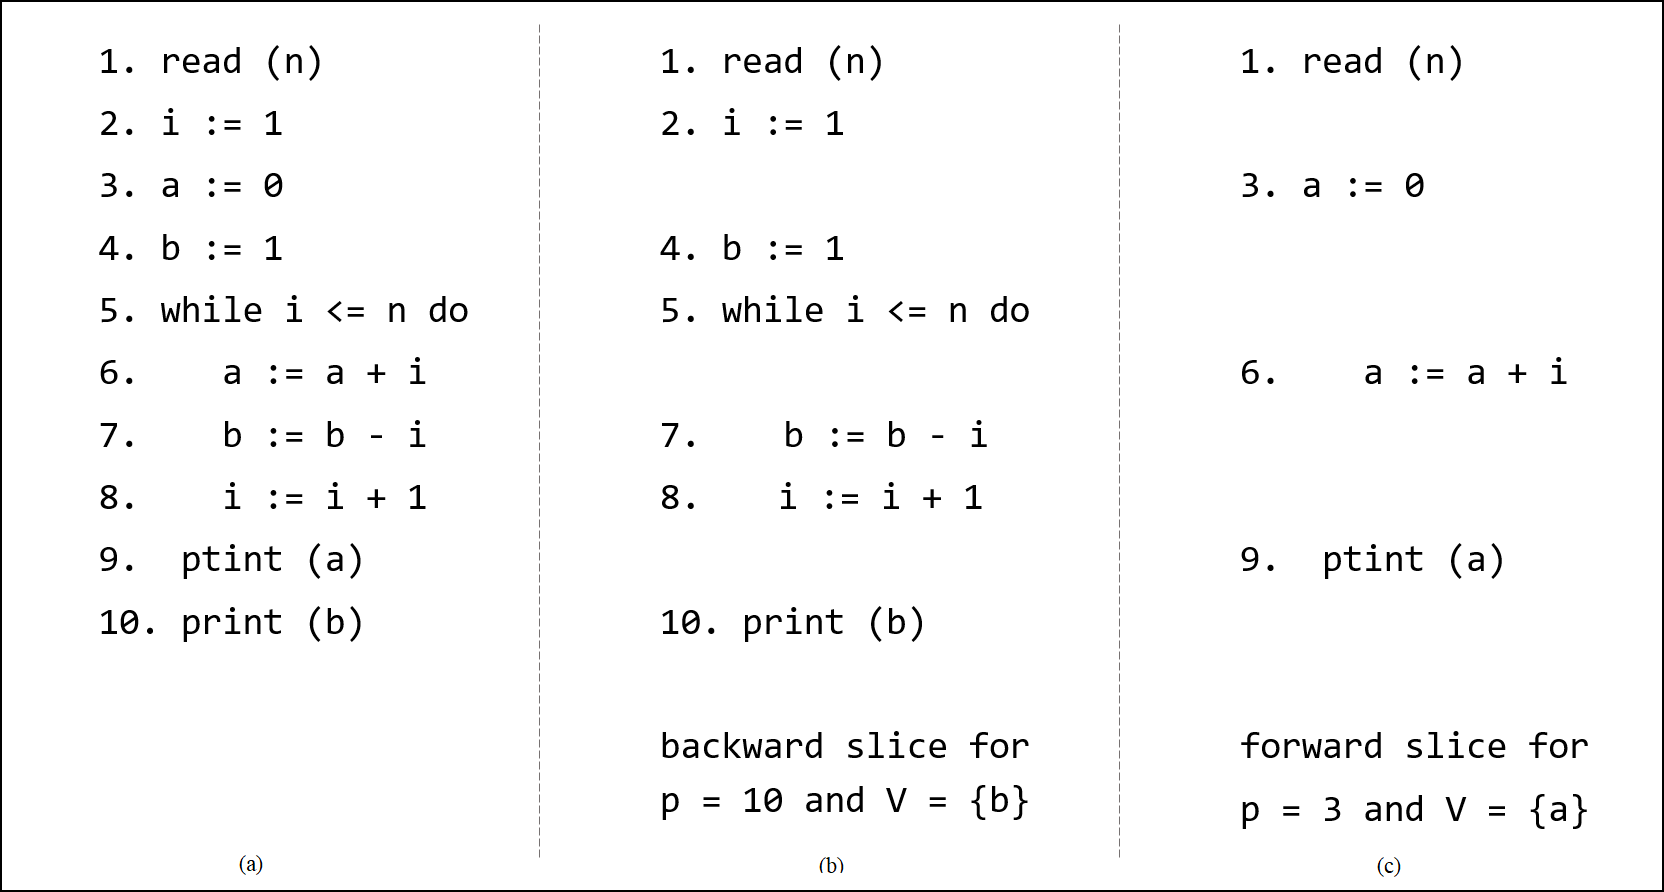
\includegraphics[width=\textwidth]{figs/exslic.png}
  %\vspace{-0.1in}
  \caption{Example of backward and forward static slicing}
  %\vspace{-0.2in}
 \label{fig:exslic}
\end{figure}

In summary, in the backward approach, the statements of the program that does not have any effect on the criterion are sliced away. However, the forward approach slices away those statements not affected by the criterion.
Our work can be viewed as a more accurate form of backwards static slicing starting from a requirement ~\cite{Tip95asurvey}. Slicing can determine the cone of influence (COI) for a given property, while IVCs are a subset of COI.

In fact, to start the verification process and IVC computation, we fisrt perform {\em backwards slicing} from the formula that defines the property of interest of the model. This step is to speed up the verification process.
 Then, IVCs are computed from the proof of the property over the sliced model.  The slice produced is smaller and more accurate than a static slice of the formula~\cite{Weiser:1981:slicing}, but guaranteed to be a sound slice for the formula for all program executions, unlike dynamic slicing~\cite{Agrawal:1990:slicing}.  Predicate-based slicing has been used~\cite{Li04:slicing} to try to minimize the size of a dynamic slice.  Our approach may have utility for some concerns of program slicing (such as model understanding) by constructing simple ``requirements'' of a model and using the tool to find the relevant portions of the model.


\section{UNSAT cores and Minimal UNSAT Subformulae}
\label{sec:muses}
Satisfiability (SAT) Modulo Theories (SMT) solvers are powerful tools to decide the
satisfiability of formulas with respect to background theories expressed in classical first order logic with equality. When using SAT solvers, instead of SMT solvers,  the language of the solver is Boolean logic and the problem must be encoded into
propositional logic.

A Boolean formula is satisfiable if there is a consistent assignment of values $true$ or $false$ to its variables in such a way that the formula evaluates to $true$. If the formula evaluates to $false$ for all possible variable assignments, then it is unsatisfiable. For example, the formula
 $a \wedge \neg a$ is unsatisfiable because there is no possible
 assignment for $a$ to make the formula
 evaluate to $true$.
 On the other hand the formula
  $a \vee b$ is satisfiable when at least
  either $a$ or $b$
  is assigned to $true$. An assignment that makes the formula $true$ is called a model. Solvers return a satisfiable model in case the formula is satisfiable: $a = true$ is one possible model for our example.

For a given unsatisfiable problem instance, solvers try to generate a proof of unsatisfiability. It is usually more useful to have a minimum proof of unsatisfiability. Such a proof is dependent on identifying a sub-set of clauses that make the problem unsatisfiable. Solvers are usually capable of reporting such sub-sets in the proof, which is known as \emph{UNSAT core}. However, the generated unsat core is not guaranteed to be minimal.

Every propositional logic formula can be transformed into an equivalent conjunctive normal form (CNF) using the laws of Boolean algebra. A formula is in CNF if it is a conjunction of clauses (or a single clause). Each clause is a disjunction of positive or negative literals (i.e., a variable or the negation of a variable). So each CNF formula can be formulated as a finite set of clauses (or constraints). Then we assume there is a function $\checksat(F)$ which determines if $F$ is satisfiable or not.
When $F$ is unsatisfiable, we assume we
have a function $\unsatcore()$ which returns a minimal subset of the
constraints such that the formula is satisfiable without them.

\begin{definition}{\emph{Minimal Unsatisfiable Subformulas(MUSes):}}
  \label{def:mus}
  Let $C$ be a finite set of constraints.
  $U \subseteq C$ be its unsatisfiable subset.
  A constraint $c \in U$ is an
  unsatisfiable core for $U$ if $U \setminus \{c\}$ is satisfiable.
  A set of all unsatisfiable cores of $U$ constitute
  an MUS for $C$.
  Note that such a set is not necessarily unique, and $C$ can have several distinct MUSes.
\end{definition}

Our work builds on top of a substantial foundation building
MUSes from UNSAT cores \cite{Cimatti2007:UNSAT}.  Recent algorithms can handle very large problems, but computing MUSes is still a resource-intensive task.  While some work is aimed at providing a set of minimal unsatisfiable formulae, minimality is usually defined such that given a set of clauses $M$, removing any member of $M$ makes it satisfiable \cite{belov2012computing}.  The step of producing minimal invariants for proofs has been investigated in depth by Ivrii et al.~\cite{Ivrii14:invariants}.

In  recent  years,  a  number  of  efficient algorithms  for  extracting minimal UNSAT subformulae (MUSes)  have  been proposed \cite{liffiton2005max},
most of which are focused on computing a single MUS  \cite{bacchus2015using, belov2012muser2, belov2013core, belov2012towards, nadel2014accelerated}. A general algorithm for extracting a single MUS is shown in Algorithm \ref{alg:mus}.

\begin{algorithm}[t]
  \SetKwInOut{Input}{input}
  \SetKwInOut{Output}{output}
  \Input{an unsatisfiable set of constraints $C$}
  \Output{MUS $M$}
  \BlankLine
  $M \leftarrow C$\\
  \For{$c \in M$} {
    \If{$\checksat(M \setminus c) = \unsat$}{
      $M \leftarrow M \setminus \{c\}$
    }
  }
  \Return{M}
\caption{SAT domain single MUS extraction algorithm}
\label{alg:mus}
\end{algorithm}

As mentioned, an unsatisfiable problem can have several distinct MUSes. Although the problem of finding all MUSes is even harder than finding one MUS, there is some strong research in the literature focusing on this problem. For example, Recent work by Liffiton et al. \cite{marco2016fast} proposed an efficient algorithm to generate MUSes, called MARCO.
Another work by Bendik et al. \cite{bendk16} tries to address this problem in the domains where minimization process is rather expensive.
These algorithms can be used in our work in order to develop a new algorithm for computing all minimal IVCs. This will require changing the underlying mechanisms that are used to construct candidate solutions and also changing the structure of the proof of correctness. The technique used in MARCO can be adapted to our work for computing all minimal IVCs. Algorithm \ref{alg:marco} is an abstract version of MARCO. This algorithm uses a symbolic representation of the
power set of $C$, $\mathcal{P} (C)$,  cleverly exploiting isomorphism between finite power sets
and Boolean algebras.
A brute-force approach to calculate all MUSes is basically explore all subsets of $C$ and determine if they are MUS or not. In the power set exploration process, subsets whose satisfiability is not known
yet are called \emph{unexplored}; i.e., initially, all subsets in $\mathcal{P} (C)$ are unexplored, and at the end, satisfiability of every subset is known; i.e., all are \emph{explored}.
In MARCO, subsets of
 $C = \{c_1 ,c_2 , \dots ,c_n \}$ are encoded using a set of Boolean variables (literals)
$A = \{a_1 ,a_2 , \dots, a_n \}$ such that every constraint $c_i \in C$ is assigned to a Boolean variable $a_i \in A$. Let assume we have a function $Lit: C \rightarrow A$ that returns a corresponding literal of $c_i \in C$.

Then the algorithm maintains a Boolean formula from literals of $A$, called $map$, to represent the set
of unexplored subsets of $C$.  $map$ is initially $true$.
MARCO iteratively explores $\mathcal{P} (C)$ to find each MUS. In each iteration, an unexplored subset $C' \subseteq C$ is non-deterministically selected by finding
a model of $map$. If $C'$ is satisfiable, it is grown
to a maximal satisfiable subset (MSS); Set $S \in C$ is MSS if $\forall c \in C \setminus \{S\}, (S \cup \{c\})$ is unsatisfiable. All subsets of a maximal satisfiable subset are also satisfiable. So, in this case, $map$ is updated in a way to block those subsets from future computation by marking them as \emph{explored} (line \ref{line:marco:sat}).
On the other hand, if $C'$ is $\unsat$, it is shrunk to a MUS.
When an MUS is found then all of its supersets are guaranteed to be unsatisfiable. So, $map$ is updated in a way
to mark all those supersets as \emph{explored} in order to block them from future exploration (line \ref{line:marco:unat}).
The grow/shrink procedure can be carried out by any algorithm for
a single MSS/MUS extraction which makes MARCO applicable to arbitrary
constraint satisfaction domain.\footnote{In Algorithm \ref{alg:marco} we abstracted these procedures. The shrink is basically the loop in Algorithm \ref{alg:mus}. A similar approach can be taken to perform the grow procedure: constraints are added one by one in a loop to check for unsatisfiability. We will explain these procedures further in Chapter \ref{ch:ivc}.}

\begin{algorithm}[t]
  \SetKwInOut{Input}{input}
  \SetKwInOut{Output}{output}
  \Input{an unsatisfiable set of constraints $C$}
  \Output{set of all MUSes $AM$}
  \BlankLine
  $AM \leftarrow \empty$
  $map \leftarrow \top$ \\
   \While{$\checksat (map) = \sat$}  {
   $C' \leftarrow$ find an unexplored subset of $C$ using a model of $map$
    \If{$\checksat(C') = \sat$}{
      $M \leftarrow$ grow $(C')$\\
      $map \leftarrow map \wedge (\bigvee_{c_i \notin M} Lit (c_i))$  \label{line:marco:sat}
    }
    \Else{
    $M \leftarrow$ shrink $(C') $\\
    $AM \leftarrow AM \cup M$ \\
    $map \leftarrow map \wedge (\bigvee_{c_i \in M} \neg Lit (c_i))$ \label{line:marco:unat}
    }
  }
  \Return{$AM$}
\caption{MARCO algorithm for computing all MUSes}
\label{alg:marco}
\end{algorithm}


UNSAT cores and MUSes are used for many different activities within
formal verification. Gupta et al. \cite{gupta2003iterative} and
McMillan and Amla \cite{mcmillan2003automatic} introduced the use of
unsatisfiable cores in proof-based abstraction engines. Their goal is
to shrink the abstraction size by omitting the parts of the design
that are irrelevant to the proof of the property under verification.
However this work is for finite systems in the domain of SAT solving,
 and the abstractions built are not intended to be returned to the user.
 We design our algorithms for IVC computation for
 infinite systems with the support of the state of the art of the SMT solvers. In addition, for IVC computation, the goal is to provide meaningful results to the user.

\section{Proof/Lemma Minimization}
\label{sec:proofcert}
The IVC idea shares many similarities with approaches for computing minimal invariant sets for inductive proofs (such as is performed for inductive proof certificates~\cite{piskac2016, Ivrii14:invariants}).
A proof certificate is an artifact embodying a proof of the
claim that can then be validated by a trusted checker.
Given a safety property $P$, an formula $Q$ is a $k$ inductive strengthening of $P$ if
$P \rightarrow Q$, and $Q$ is $k$ inductive.
%For $i = 1,2$, if $Q_i$ is $k_i$
%inductive strengthening of $P_i$, then $(Q_1 \wedge Q_2)$
%is $k$ inductive strengthening of $(P_1 \wedge P_2)$, where $k = max(k_1, k_2)$.
Formula $Q$ is a certificate for property $P$ if $Q$ is
a $k$ inductive strengthening of $P$.
Certificates need to be concise and efficient to check
by an independent tool or method. In particular,
checking a certificate should not take more
time than proving the original property. Mebsout and Tinelli presented a method for extracting and verifying proof certificates \cite{piskac2016} implemented in \texttt{Kind 2} model checker.
\texttt{Kind 2} performs verification by running different engines concurrently. Specifically, it employs number of auxiliary invariant generation engines to
discover and pass along auxiliary invariants that might be
helpful in proving a property of interest. Then these invariants are considered as
safety certificates for the property.
To simplify the certificates, they either reduce $k$ or the size/complexity of the certificate formula.
After obtaining a $k$ inductive invariant $Q$, \texttt{Kind 2} starts with reducing $k$ before simplifying the formula. It will replay the inductive
step for $Q$ for values $i < k$ , following one
of three different strategies:
\begin{itemize}
  \item forward enumeration: all values of $1 \le i \leq k' < k$  are checked, and $k'$ is the first where $k'$ inductiveness holds.
  \item binary search: the interval $[1 , k ]$ is divided into
  subintervals $[1 , k' ]$ and
$[ k' + 1 , k ]$ of similar size. Then, the first or
the second interval is recursively considered depending on whether $Q$ is $k'$ inductive
or not.
  \item backward enumeration: all values of $i$ from $k$ down to 1 are checked, and it stops
when $k'$ inductiveness does not hold anymore.
\end{itemize}

To simplify the certificate, $Q$ is converted into a set of subformulae.
Iteratively, each subformula is removed from a set and it is checked if $Q$ is still $k$ inductive or not. In this case subformulae not needed to prove
$Q$ are pruned away. Finally, to verify a certificate, it needs to be proved that $Q$ is
a $k$ inductive strengthening of the original property.

Our IVC algorithm also needs to find a minimal lemma set.  However, there is a substantive difference: to find a minimal set of constraints, it is usually necessary to find new proofs involving {\em new lemmas} not used in the original proof, which accounts for the expense of finding an accurate minimal IVC. This process will be explained in Chapter \ref{ch:ivc}.
%Note that our lemma minimization technique used in IVC generation is actually more efficient than the above technique.


\section{Traceability}
\emph{Requirements traceability} can be defined as

\begin{quotation}
\textit{``the ability to describe and follow the life of a requirement, in both forwards and backwards direction (i.e., from its origins, through its development and specification, to its subsequent deployment and use, and through all periods of on-going refinement and iteration in any of these phases).''}~\cite{gotel}.
\end{quotation}

Traceability has been of great interest in research and practice for several decades. Intuitively, it concerns establishing relationships, called \emph{trace links}, between the requirements and one or more artifacts of the system.
Among the several different development artifacts and the relationships that can be established from/to the requirements, being able to establish trace links from requirements to artifacts that realize or \emph{satisfy} those requirements---particularly
to entities within those artifacts called \emph{target artifacts}~\cite{gotel2012traceability}---has been enormously useful in practice. For instance, it helps analyze the impact of changes in one artifact on the other, assess the quality of the system, aids in creating assurance arguments for the system, etc. In this work, we focus our attention on a subset of requirements traceability that we call \emph{Requirements Satisfaction Traceability.}

Instead of just recording the trace links from each requirement to the target artifacts, \emph{Satisfaction Arguments}~\cite{zave1997four} offer a semantically rich way to establish them. Originally proposed by Zave and Jackson~\cite{zave1997four}, a satisfaction argument demonstrates how the behaviors of the system and its environment together satisfy the requirements. From a traceability perspective, these arguments help establish
 trace links (the \emph{satisfied by} relationship) between the requirements and those parts of the system and environment (the target artifacts) that were necessary to satisfy the requirements; We call those target artifacts a \emph{set of support} for that requirement. This set of support is the same as a minimal inductive validity core obtained from the correctness proof of the requirement.

\section{Requirements Adequacy}
Determining adequacy of properties has also been extensively studied. Certification standards such as DO-178C~\cite{DO178C} require that requirements-derived tests achieve some level of structural coverage (MC/DC, decision, statement) depending on the criticality level of the software, in order to approximate adequacy.  If coverage is not achieved, then additional requirements and tests are added until coverage is achieved. Recent work by Murugesan~\cite{murugesan2015we} and Schuller~\cite{schuler_assessing_2011} attempted to combine test coverage metrics with requirements to determine completeness.  Chockler~\cite{chockler_coverage_2003} defined the first adequacy (completeness) metrics directly on formal properties based on mutation coverage.  Later work by Kupferman et al.~\cite{Kupferman:2006:SCF} defines completeness as an extension of vacuity to elements in the model.  We present an alternative approach that uses the proof directly, which we expect to be considerably less expensive to compute.


\subsection{Coverage and Mutations}

Different notions of coverage have been defined in software testing. However, in formal verification, it is not immediately obvious how to define and compute coverage.
%Usually, coverage techniques in the property-based verification try to measure the quality of the specification in regard to the completeness of a set of properties.

Coverage in verification was introduced in \cite{hoskote1999coverage, katz1999have}. Hoskote et al. \cite{hoskote1999coverage} suggested a state-based metric in model checking based on FSM mutations, which are small atomic changes to the design. Then, the method for measuring coverage is to model check a given property for each mutant design.
Later in \cite{chockler_coverage_2003}, Chockler et al. provided corresponding notions of metrics used in simulation-based verification for formal verification. In fact, they improved the same idea of mutation-based coverage where each mutation is generated to check if a specific
design element is necessary for the proof of the property.
 However, the proposed algorithm is both computationally expensive: each mutant model must be separately analyzed, which can easily lead to tens of thousands of verification problems on models of moderate size. Note that most of the mutation-based metrics, including \cite{kupferman_theory_2008, chockler2001practical}, are focused on finite state systems and hardware systems.
In general, specification completeness can be defined with
regard to the notion of coverage. In fact, the way that coverage
is formalized plays a key part in the strength/ effectiveness of
a method for the assessment of completeness.

The goal of a coverage metric is usually to assign a numeric score that describes how well properties cover the design. The majority of the work on coverage metrics has focused on {\em mutations}, which are ``atomic'' changes to the design, where the set of possible mutations depends on the notation that is used.  A mutant is ``killed'' if one of the properties that is satisfied by the original design is violated by the mutated design~\cite{chockler_coverage_2003,chockler2001practical,chockler2010coverage,Kupferman:2006:SCF,kupferman_theory_2008}.  There are many different kinds of mutations that have been proposed, primarily focused on checking sequential bit-level hardware designs.  For these designs, {\em state-based} mutations flip the value of one of the bits in the state.  There are several variations depending on whether the flip is performed on a single state within a Kripke structure~\cite{hoskote1999coverage}, or in the description of the signal in the transition relation of the circuit~\cite{chockler2001practical}.  {\em Logic-based} mutations fix the value of a bit to constant zero or one, and can be used to determine whether properties can find stuck-at faults.  {\em Syntactic} mutations~\cite{chockler_coverage_2003} remove states in a control flow graph representation of hardware.  Similarly, for software, it is possible to apply any of the ``standard'' source code mutation operators used for software testing~\cite{Andrews06:mutation} towards requirements coverage analysis.  Some examples of software mutations are \cite{Budd:1980}:
\begin{enumerate}
    \item Replace an integer constant $C$ by one of $\{0, 1, -1, C + 1, C - 1\}$,
    \item Replace an arithmetic, relational, logical, bitwise logical, increment/decrement, or arithmetic-assignment operator by another operator from the same class,
    \item Negate the decision in an \texttt{if} or \texttt{while} statement,
    \item Delete a statement.
\end{enumerate}

Mutation-based approaches are often impractically expensive to compute; even for small models, there are many possible mutations and we deal with too many verification problems.  The number of single-mutation programs is roughly the product of the leaf elements of the program abstract syntax tree (AST) and the size of the chosen set of mutations, which can lead to an impractical number of verification problems.

\newcommand{\andnode}{{\sc and}}
\newcommand{\invnode}{{\sc inv}}
\newcommand{\inpnode}{{\sc inp}}
\newcommand{\regnode}{{\sc reg}}
\newcommand{\mutnode}{{\sc mut}}
\newcommand{\inputnode}{{\sc input}}

Mutations for hardware are discussed in~\cite{chockler2010coverage,Kupferman:2006:SCF,kupferman_theory_2008}. A more recent work in \cite{chockler2010coverage} performs coverage analysis through interpolation \cite{mcmillan2003interpolation}. This work is also based on design-dependent mutations \cite{chockler_coverage_2003}, where a design is considered as a net-list with nodes of types \{ \andnode, \invnode, \regnode, \inputnode \}.
Each mutant design changes the type of a single node to \inputnode .
%When property $\phi$ satisfied by the original net-list fails on the mutant design, it is said that a mutant is discovered for $\phi$.
%Then, the coverage metric for $\phi$ is defined as the fraction of the discovered mutants, based on which the coverage of a set of properties is measured as the fraction of mutants discovered by at least one property.
To decrease the cost of computation, coverage analysis is performed at several stages; first, all the nodes that do not appear in the resolution proof of a given property are marked as \emph{not-covered}, and the rest of the nodes are marked as \emph{unknown}. Then, for the unknown nodes, the basic mutation check is performed: if a corresponding mutant design violates the property, it will be considered as \emph{covered}. Otherwise, the algorithm tries to drive an inductive invariant to prove that the node is not covered. Finally, an interpolant-based model checking is applied to the nodes that are still unknown.

Most of the mutation-based coverage techniques can be put into the category of falsity coverage, where we mutate the design and see if the property is still valid or not.
In this way, we understand if that mutant was necessary (covered) for (by) that property.
It is important to note that some mutations yield a subset of the state space of the system to
be explored; in this case, any universal property that was true of the original system
must, by definition, be true of the mutated system. This is where falsity coverage is not effective, and the notion of \emph{vacuity coverage} comes into play. Falsity coverage asks weather the mutant FSM still satisfies the property, while vacuity coverage checks if the mutant FSM satisfies the property vacuously. In vacuity coverage, first, we makes sure the property is non-vacuous. Then, we mutate the design. If the property is
vacuous afterwards, it means that the mutant was necessary for that property.


%\mike{end placement}

A similar notion to IVCs outlined in a patent~\cite{hanna2015formal}, which sketches a family of {\em proof core}-based metrics for use in hardware verification.  While the approach described by the patent is general, it is quite underspecified and it is not possible to compare their approach and ours. In addition, in commercial hardware verification frameworks do different forms of coverage analysis: Cadence JasperGold~\cite{jasper_gold} does some form of proof core coverage and Synopsys VC Formal~\cite{Synopsys_VC_formal} does a mutation-based coverage approach.  These coverage measurement approaches may be similar to the metrics we introduce but are not described in sufficient depth to be compared.

A different approach to measure coverage involves checking whether each output signal is fully constrained by the specification \cite{das2005formal, claessen2007coverage, grosse2007estimating}. For example, in \cite{claessen2007coverage}, authors propose a design-independent coverage analysis where missing properties are identified by unconstrained output signals. Given a property list and a specific computed signal $s$ (usually drawn from the circuit outputs), if there is a trace with a point in time when $s$ is not constrained to be a single value by the set of properties and the input trace, then the property set is incomplete. Alternately, given two traces that differ only in the value of signal $s$ at a particular time step, if both traces satisfy property $P$, then $s$ is not covered by $P$.
 The work in \cite{haedicke2012guiding} refines this notion of coverage by providing a numeric score for each incompletely covered signal $s$.  Such metrics are very rigorous but can lead to overspecification: the specification must completely define the input/output function of the implementation.

%a coverage metric that computes a numerical value to describe how much of the circuit behavior is constrained by a given set of properties. This methods investigates, given property $\phi$ and a specific output $s$, if there exist two traces $\sigma_{1}$ and $\sigma_{2}$ that: (1) $\sigma_{1} \vDash \phi$ and $\sigma_{2} \vDash \phi$ (2) $\forall$ signals $s' \neq s, \forall t. \sigma_{1}(t, s') = \sigma_{2}(t, s')$ (3) $\exists t. \sigma_{1}(t, s) \neq \sigma_{2}(t, s)$. This method was implemented in SMV model checker \cite{smv}.

Another technique to measure requirements completeness is to employ several surrogate models; for example, Zowghi and Gervasi~\cite{zowghi2003three} use refinement to show {\em relative completeness} with respect to a {\em domain} model, which describes the behavior of the real world, irrespective of change induced by software.  In their model, each iteration of refinement of requirements and domain models must be sufficient to prove the requirements of the previous iteration.  However, this idea has two problems: first it provides no notion of absolute completeness, and second, it requires construction of a domain model, which is often difficult and/or expensive to construct.

Outside the context of formal verification, many authors have theorised and empirically validated conceptual model completeness, which are mostly dependent on a subjective judgement \cite{drechsler2012completeness, firesmith2005your, chang2007finding,katta2013investigating, zowghi2003three, espana2009evaluating}.



\section{Vacuity Detection}
Another potential use of our work is for ``semantic'' vacuity detection.  A standard definition of vacuity is syntactic and defined as follows~\cite{Kupferman:2006:SCF}: {\em A system K satisfies a formula $\phi$ vacuously iff $K \vdash \phi$ and there is some subformula $\psi$ of $\phi$ such that $\psi$ does not affect $\phi$ in K}.  Vacuity has been extensively studied~\cite{Gurfinkel:2012:RVB,Chockler2008,DBLP:Ben-DavidK13,Kupferman:2006:SCF,Chockler:2007,Beer1997} considering a range of different temporal logics and definitions of ``affect''.  On the other hand, our work can be used to consider a broader definition of vacuity.  Even if all subformulae are required (the property is not syntactically vacuous), it may not require substantial portions of the model, and so may be provable for vacuous reasons.  The problem is exacerbated when the modeling and property language are the same (as in JKind), because whether a subformula is considered part of the model or part of the property, from the perspective of checking tools, can be unclear.

Torlak et al. in~\cite{Torlak08:cores} finds MUSes of Alloy
specifications, and considers semantic vacuity.
 Alloy models are only analyzed up to certain
size bounds, however, and in general are unable to prove properties
for arbitrary models. Also, because we are extracting information from
proofs, it is possible to use IVCs for additional purposes (proof
explanation and completeness checking).

\section{Safety Standards}
Due to the complexity of computer systems and our reliance on them, it is of the utmost importance that the development of these systems proceeds in a way that minimizes development errors. There are a several safety standards that focus on safety critical components, including DO-178C \cite{DO178C}, MOD-0053 \cite{standard2007standard}, and ISO 26262 \cite{iso201126262}. Production of a functional safety case is usually a requirement for compliance with a specific standard, which brings opportunities and challenges to safety practitioners and researchers. In this section we briefly describes the objectives of these standards and how IVCs can be related to this area.

Software Considerations in airborne systems and equipment are usually regulated by certification: the DO-178C standard \cite{DO178C}.   There are a couple of key components in DO-178C that are related to our purpose; first is to ensure the low-level requirements are in compliance with the high-level safety requirements. That is, each refinement must be shown not to introduce functionality not present in the artifact from which it was derived (adequacy).
Another component of DO-178C is coverage analysis at the two levels: requirements-based analysis and structural analysis.
After requirements-based testing, which ensures the software in the target computer will satisfy the high-level requirements, the purpose of coverage analysis in DO-178C is to determine how well this type of testing verified the implementation of the software requirements. Then, the structural coverage analysis is to determine which code structure was not exercised by the requirements-based test procedure.
DO178C  uses a variety of metrics to determine adequacy of requirements, but much of the effort involves code-level testing.  Test suites are derived from requirements and used to test the software, then measured using different structural coverage test metrics.
If code-level test suites do not achieve full coverage, then an analysis is performed to determine whether there are missing requirements and test cases.  The kind of structural coverage required (e.g., statement, branch, MCDC) for adequate testing is driven by the criticality of the software in question.
Traceability is another explicitly defined component of DO-178C; that is, low-level requirements must be traceable to the high-level requirements that they refine. Further, two other traceability objectives in DO-178C are (1) traceability of high-level requirements to system requirements and (2) traceability of software design to high-level requirements, which specifically require applicants to demonstrate bi-directional traceability.

MOD-0053 \cite{standard2007standard} is a defense standard that provides safety management requirements for defense systems, which are designed to be applied in different phases of the development process of MOD\footnote{Ministry of Defence} projects. A key component of this standard is a
\emph{Safety Case}, which demonstrates how safety will be achieved and maintained. To summarize a Safety Case and document safety management activities, Safety Case Reports should be provided. These reports describe a structured argument that the system is acceptably safe. Hazard analysis is another important component of MOD-0053, for which enough evidence must be provided to show all hazards are identified and properly managed. Therefore, traceability in this standard is a key component defined at two levels: (1) traceability  between each safety
requirement and the source of that requirement, and (2) traceability of the safety
risk/hazards management to hazards and accidents. Requirements traceability in MOD-0053 should be established in both ways: (1) to trace each requirement to the
part of the code which implements it, and (2) to trace from any part of the
code, back through the software design/specification, to the requirement. Currently, traceability checks are performed via traceability matrices built manually, however, MOD-0053 recommends that traceability be provided between the formal arguments and the software
requirement, which will help to check if all the requirements have
been verified, and to ensure that the implications of changes to requirements can be assessed. In addition to traceability, this standard requires an assessment of the veracity and completeness of the software Safety Case.  We believe that many of these traceability and adequacy checks can be automated using IVCs.

ISO 26262 \cite{iso201126262} is a common standard used in the automotive industry whether an automotive system is acceptably safe. This standard provides guidance in different steps of the product development process to manage functional safety of a system at the hardware and software levels.
One important component of ISO 26262 is Automotive Safety Integrity Levels (ASILs), by which each component is assigned to an acceptable risk level determined at the beginning of the development process. The goal is to analyze the system functionalities with respect to possible hazards. Each requirement is assigned a class of criticality from A to D, where D has the most safety critical processes and strictest testing regulations. In ISO 26262, qualification of software components demand testing not only under normal operating conditions, but also in the presence of faults so to determine how system reacts to abnormal inputs.  ISO 26262 has other important components like \emph{test tool qualification}, which are not closely related to the context of verification.

In order to meet the objectives of the safety standards, developers have to put a lot of manual effort into providing acceptable evidence such as assurance cases, traceability matrices, and requirements adequacy. We claim that some of these safety analyses can be automated with the IVC notion, and we would like to study how we can achieve that. Since IVCs are derived from the formal proofs, they will make much more accurate safety evidence than those created manually.

